\documentclass{article}
\usepackage{parskip}
\usepackage{graphicx}
\usepackage{caption}
\captionsetup{justification=raggedright, singlelinecheck=false}
\graphicspath{ {./fragments/desktop/} }
\title{Final Report}
\author{By Project Prime}
\begin{document}
 \maketitle
 \section{\underline{Introduction}}
In this project, we were tasked with building a multi-host file synchroniser consisting of three components: a server, a mobile client and desktop client. The server is the \textit{hub} while the clients are the \textit{spokes}. The server was created using Node.js, where it adopted the role of an interface between the clients and MongoDB database. In addition, the server is stored in the Heroku cloud platform to provide both clients with universal file access and processing. The Node.js server can also process HTTP requests to allow both clients to upload, delete and download files. The mobile client was developed using Java and XML on Android Studio, whereas the desktop client was developed using Javascript, HTML and CSS on Electron. The output of the project is a fully-functioning file synchroniser that interacts with both clients via the Node.js server. This project addresses the problem of long durations to complete tasks; thus, the solution will take the form of two clients that minimise the duration to complete tasks as low as possible.

\section{\underline{Review}}
\subsection{\underline{Server Application}}

\subsection{\underline{Desktop Client}}
The common file hosting service, Dropbox, uses a method which they call “Sync” to keep its files updated across mobile and desktop clients. Its split into two stages: upload and download.
Once a file is uploaded through the server, it is added to their database before other clients are notified of its existence. According to (Koorapati, 2014), the host client does not use a traditional file system directory and allocates a namespace for each user. Their metadata database also known as the Server File Journal stores this information and connects directly to one of Dropbox’s server types: Metadata Server. The actual contents of the file are stored in block data servers. The advantage of having a separate database for the metadata here is that the main contents of the files are less vulnerable to threats because they won’t need to be referenced as often as the metadata for reviewing updates about the files. Furthermore, a good file synchronisation software is defined by how robust its security is and their block data servers are all encrypted using “256-Bit Advanced Encryption Standard” as mentioned in (Dropbox, n.d). 
Therefore, the protocol described in (Koorapati, 2014) for Dropbox’s desktop client is as follows:
\begin{itemize}
\item The upload client commits to the metadata server first to check if there exists a namespace for the file stored in the block server already.
\item For new files, the metadata server would return “need blocks” and the client then directly talks with the block data server to store the new file.
\item The process is repeated and any updates to the file can be checked by only talking to the metadata server.
\item To download a file, the downloading client pings the metadata server to retrieve a list of updates. The Server File journal notifies the client that a new file was added.
\item The download client now contacts the block data server directly to access the new file.
\end{itemize}
This protocol shows that both the desktop client and server application in Dropbox are equally involved in the synchronization process. However, this is not always the case in other software, for example Unison, an open-source file sync. 

\subsection{\underline{Mobile Client}}

\section{\underline{Requirements and Design}}
Requirements have been derived for each component. The requirements have been analysed using the MoSCoW prioritisation technique (Madsen, 2017); as a result, each requirement has been placed into one of the following categories: \textit{Must Have} (critical requirements with the highest priority), \textit{Should Have} (important but unnecessary requirements for the final product), \textit{Could Have} (lowest-priority requirements that would be implemented if time permits) and \textit{Won't Have} (least critical requirements that are unrequired for project success). In addition, the subsections will show the designs that reflect the corresponding component.

\subsection{\underline{Desktop Client}}
\begin{tabular}{|p{3cm}|p{5cm}|p{4cm}|}
\hline
\multicolumn{3}{|c|}{\textbf{MoSCoW requirements for The Desktop Client}} \\
\hline
\textbf{Requirement No.} & \textbf{Requirement} & \textbf{Priority}\\
\hline
1 & Must be able to communicate with the Server Application & Must Have \\
\hline
2 & Has to be able to upload files & Must Have \\
\hline
3 & Has to be able to download files from database via server & Must Have \\
\hline
4 & Make use of a file management system to upload any file from the user's system & Must Have \\
\hline
5 & Check for updates regularly so that the desktop client is in sync with the Server and Mobile Client & Must Have\\
\hline
6 & Display the current list of files from the database in the centre of the page & Should Have \\
\hline
7 & Include a delete file functionality   & Should Have \\
\hline
8 & Provide a way to track and check recent changes to files & Could Have\\
\hline
9 & Include a search bar to quickly find files if the list of files is too large & Could Have \\
\hline
10 & Have User profiles for personalised access & Won't Have \\
\hline
\end{tabular}

\subsection{\underline{Mobile Client}}
\begin{tabular}{|p{3cm}|p{5cm}|p{4cm}|}
\hline
\multicolumn{3}{|c|}{\textbf{MoSCoW requirements for The Mobile Client}} \\
\hline
\textbf{Requirement No.} & \textbf{Requirement} & \textbf{Priority}\\
\hline
1 & Must be able to communicate with the Server Application & Must Have \\
\hline
2 & Must be able to upload files into the database through the server & Must Have \\
\hline
3 & Must be able to delete files & Must Have \\
\hline
4 & All changes must be reflected in the files stored in the server & Must Have \\
\hline
5 & The mobile UI must be simple and easy to navigate through & Should Have \\
\hline
6 & All the application's functions should be accessible from the main page & Should Have \\
\hline
7 & All files files should be listed with both filename and time of last modification clearly visible to the user & Should Have \\
\hline
8 & Include a search bar to quickly search through the list of files & Could Have \\
\hline
\end{tabular}

\subsection{\underline{Server Application}}

\begin{tabular}{|p{3cm}|p{5cm}|p{4cm}|}
\hline
\multicolumn{3}{|c|}{\textbf{MoSCoW requirements for Server Application}} \\
\hline
\textbf{Requirement No.} & \textbf{Requirement} & \textbf{Priority}\\
\hline
1 & Has to be connected to a database in order to store and retrieve files & Must Have \\
\hline
2 & Must be able to communicate with the Desktop and Mobile Clients simultaneously & Must Have \\
\hline
3 & Use HTTP requests to send data to the clients & Must Have \\
\hline
4 & Handle conflicts using Rsync & Should Have \\
\hline
5 & Use security encryption to protect the data & Could Have\\
\hline
\end{tabular}

\section{\underline{Implementation}}
\subsection{\underline{Server Application}}
The server was developed using Node.js and the database used is a cloud service by MongoDB. The Node.js server is stored in the Heroku cloud platform.

\begin{tabular}{|p{2cm}|p{2cm}|p{3cm}|p{3cm}|p{3cm}|}
\hline
\multicolumn{5}{|c|}{\textbf{Test Cases for Server Application}} \\
\hline
\textbf{Test ID} & \textbf{Test Name} & \textbf{Expected} & \textbf{Actual} & \textbf{Pass/Fail/Solved} \\
\hline
1 & ... & ... & ... & ... \\
\hline
\end{tabular}

\subsection{\underline{Desktop Client}}
The desktop client was developed using  HTML, Javascript and CSS on Electron. Electron provides pre-written HTML code (Electron, n.d.) that creates a basic desktop app; the pre-written code was used as the foundation for the development of the desktop client. Afterwards, the client's front-end was modified using JS, HTML and CSS to reflect the project designs. On to the desktop client's front-end, Bootstrap CSS files and JS scripts (Bootstrap, n.d.) were also included to add and format certain elements (e.g. file upload bar and button), along with CSS files written by the desktop subgroup.
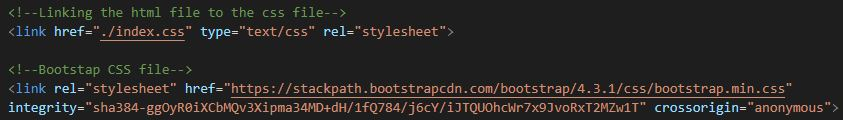
\includegraphics[width=12cm, height=2cm]{BootstrapCSSfiles}

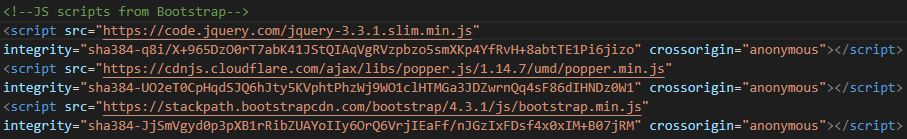
\includegraphics[width=12cm, height=2cm]{BootstrapJSscripts}

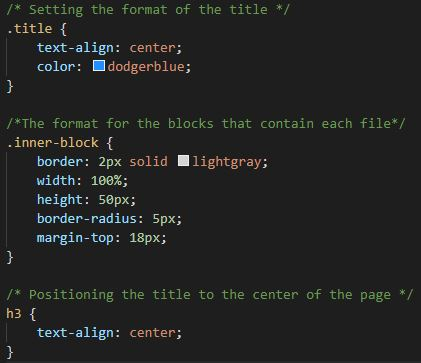
\includegraphics[width=8cm, height=6cm]{css}

After setting the foundation, the desktop subgroup concentrated on displaying files that resided in the database. To do so, the server would return a JSON object (which contains each file in the database) after a connection was formed between the desktop client and server. Using a loop, the object was traversed through and for every file encountered, that file would be presented on the client's UI. In addition, each file would be encapsulated in a file container (presented as a grey-bordered box).

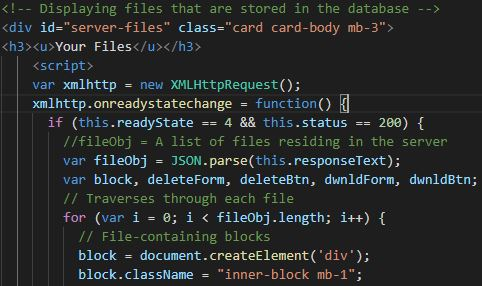
\includegraphics[width=12cm]{display1}

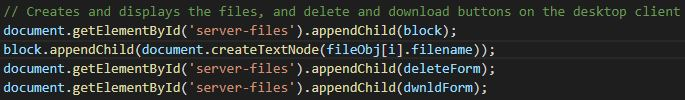
\includegraphics[width=12cm]{display2}

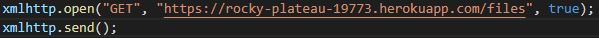
\includegraphics[width=12cm]{display3}

Next, the subgroup wrote code that enabled the client to upload files into the database via the server. After pressing the \textit{Browse} button, the local host's file manager opens, which enables the user to choose a file and subsequently, the label of the file upload bar changes to the name of the selected file; therefore, indicating which file was selected by the user. Afterwards, the user would press the \textit{Submit} button which transmits a http post request to the server, which causes the latter to store the selected file inside the database. In addition, the label of the file upload bar will revert to its initial form (i.e. "Choose a File...") after the \textit{Submit} button is pressed. 

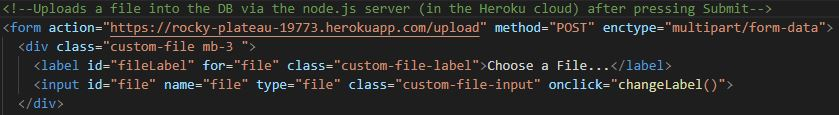
\includegraphics[width=12cm]{upload}

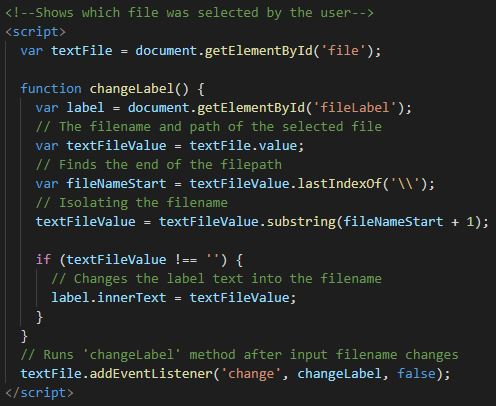
\includegraphics[width=12cm]{upload2}

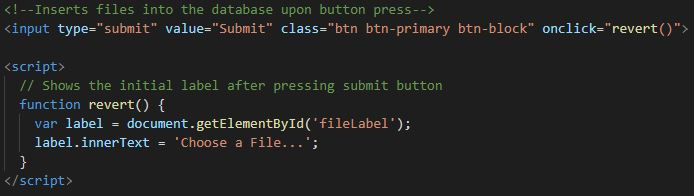
\includegraphics[width=12cm]{upload3}

Moving on to file deletion, the desktop subgroup wrote code that enabled the client to delete files; as a result, removing the corresponding document from the database. To add to this, deleting a file resulted in removing that file from the list of documents displayed on the client's UI. After pressing the \textit{Delete} button, the client would send a delete request to the server and this request would include the file's unique ID; therefore, the use of unique identification ensures the prevention of multiple files of the same name being deleted, for example. 

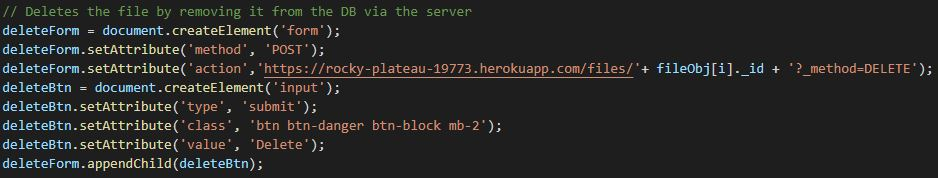
\includegraphics[width=12cm]{delete}

Finally, the desktop subgroup wrote code that enabled the client to download files from the database; as a result, bringing the corresponding document into the storage of the local host. After pressing the \textit{Download} button, the client sends a GET request to the server, which causes the server to return the file in the local host's file manager and the user stores the file in the local host's storage by pressing the \textit{save} button of the file manager. 

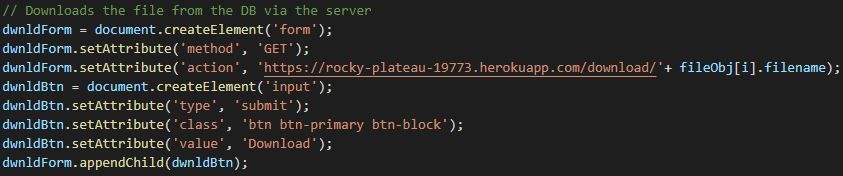
\includegraphics[width=12cm]{download}

\begin{tabular}{|p{2cm}|p{2cm}|p{3cm}|p{3cm}|p{3cm}|}
\hline
\multicolumn{5}{|c|}{\textbf{Test Cases for Desktop Client}} \\
\hline
\textbf{Test ID} & \textbf{Test Name} & \textbf{Expected} & \textbf{Actual} & \textbf{Pass/Fail/Solved} \\
\hline
1 & Connection to server & A JSON object will be returned to indicate the connection between the server and client.  & As expected & PASS \\
\hline
2 & Display file(s) & Display files stored in the Mongo database. & As expected & PASS \\
\hline
3 & Upload file & A file gets uploaded into the database via server after pressing the \textit{Submit} button. Next, the file is displayed in the list of documents stored in the server. & File was uploaded but does not appear in the list unless the page is refreshed. & 1/2 \\
\hline
4 & Delete file & A file gets removed from the database via server after pressing \textit{Delete} button. Next, the list of documents is displayed without the deleted file. & File was deleted but isn't removed from the list unless the page is refreshed. & 1/2 \\
\hline
5 & Download file & A file gets downloaded into the local host after pressing the \textit{Download} button. & As expected & PASS \\
\hline
\end{tabular}

\subsection{\underline{Mobile Client}}
The mobile client was developed using Android Studio; thus, the implementation primarily involved Java and XML.

\begin{tabular}{|p{2cm}|p{2cm}|p{3cm}|p{3cm}|p{3cm}|}
\hline
\multicolumn{5}{|c|}{\textbf{Test Cases for Mobile Client}} \\
\hline
\textbf{Test ID} & \textbf{Test Name} & \textbf{Expected} & \textbf{Actual} & \textbf{Pass/Fail/Solved} \\
\hline
1 & ... & ... & ... & ... \\
\hline
\end{tabular}

\section{\underline{Teamwork}}
Project Prime consists of six members: Yusaf, Sandipan, Saloni, Shefali, Cameron and Manny. To balance the workload, the team was divided into three subgroups of two teammates and each subgroup was assigned to the development of one component. As a result, Yusaf and Sandipan were assigned to the desktop client, Saloni and Shefali were assigned to the server, and Manny and Cameron were assigned to the mobile client. Within these subgroups, the work was distributed between both teammates through discussion. Despite the team division, members from other subgroups were permitted to intervene in the development of a component that they weren't assigned to, in order to fix issues that the assigned subgroup couldn't correct, for example. Moving onto communication, the team remotely communicated using an instant messaging app (i.e. Whatsapp), which allowed arrangements of group sessions at a certain date-and-time, notifying teammates of open pull requests, etc. Furthermore, the sessions were conducted in booked study rooms at least once per week and these sessions involved group discussion and coding of all components. Next, the project involved Github, where the project implementation was contained in a public repository called \textit{Project Prime Dev}. In addition to Git, the team followed the feature branch workflow, where a component feature was developed inside a branch seperate to the master branch and subsequently, the former would be merged into the latter branch.

\section{\underline{Evaluation}}
To start with what went well, one positive aspect was the firm strength of team communication, as all members proactively shared their thoughts and concerns in physical meetings and in the WhatsApp group. In addition, communication was carried-out in a respectful manner at all times; thus, there were no verbal conflicts during the project. Another positive aspect was the fairness in workload distribution by creating subgroups that were assigned to the development of a specific component. The rationale behind the formation of subgroups was to avoid the possibility of one member feeling overwhelmed from having lots of work. Furthermore, by assembling subgroups, this influenced the members of the subgroup to cooperate together to build the component; thus, being in a subgroup generated a sense of teamwork. Finally, a notable positive aspect was our ability to adapt to changing circumstances. For instance, it was initially planned to store files in a SQL database. Unfortunately, we discovered SQL databases were unideal for file storage since it is limited by file size. In response, we decided to migrate to MongoDB, which is a cloud service that allows the creation of document-oriented database systems that can contain files of any size.

\noindent Moving onto what didn't go well, our initial plan was weak as we didn't know how to approach the task, due to having no experience in developing file synchronisers. Although we met various project objectives, our commitment to the plan was low, as we rarely compared our progress to the initial plan during our weekly meetings. Another negative was the poor interactive feedback of certain features in particular components. For example, after pressing the \textit{Browse} button in the desktop application, there is no feedback (e.g. temporary colour change, mouse cursor change) to indicate the button-pressed.

\noindent Relative to the initial plan, there were differences between the rough timetable and actual progress. For instance, instead of using an SQL database, we decided to create and use a MongoDB database since it's document-oriented and has the capability to store files of any size, whereas SQL storage is limited by data type and size, and it cannot process text files properly; thus, with MongoDB being more suited to our needs, we abandoned the plan to use an SQL database and shifted to MongoDB instead.

\noindent On to how the team worked together, the team was divided into three subgroups as initially planned, where each subgroup developed one component of the file synchronising system; as a result, the workload was divided fairly amongst all members. Throughout the majority of the project's lifetime, the team attended group meetings once per week where group discussion and coding was conducted. Along with group meetings, communication was also conducted in a whatsapp group where we scheduled groups meetings in booked study rooms at a certain date-and-time, notified each other about opened pull requests, reminders about incomplete work, etc. The reason for choosing whatsapp as our main form of remote communication was due to everyone's familiarity with the app and its simplicity (in terms of usability); thus, there was no need to use Skype since the team was comfortable with using whatsapp, in contrary to the original plan. Despite developing the system outside the meetings, one major weakness was scheduling meetings once per week since it delayed the completion of work, which could have been completed faster if we met more than once per week by completing tasks together. Overall, the team worked well together, as there were no conflicts and each member contributed their unique  skills to the group. For instance, since Yusaf possessed leadership experience, he was elected as team leader to command the group, ensure each member's involvement in the project's activities, etc.

\noindent In conclusion, this project caused the realisation that despite our computer science backgrounds, our technical prowess is still very basic and there is much for us to learn. In response to this discovery, we will commit to thoroughly relearning and practising how to use different technologies in our spare time, including programming languages and Git (e.g. BitBucket). In retrospect, if this project was repeated, our different approach would be to partner stronger members with novice ones, in terms of technological skill; thus, providing novice members with the opportunity to enhance their skills by learning whilst working on the job.   

\section{\underline{Peer Assessment}}
\begin{tabular}{|p{2cm}|p{2cm}|p{2cm}|p{2cm}|p{2cm}|p{2cm}|}
\hline
\multicolumn{6}{|c|}{\textbf{Peer Assessment of Project Prime}} \\
\hline
\textbf{Yusaf} & \textbf{Sandipan} & \textbf{Saloni} & \textbf{Shefali} & \textbf{Cameron} & \textbf{Manny} \\
\hline
17.5 & 16.5 & 16.5 & 16.5 & 16.5 & 16.5 \\
\hline
\end{tabular}
	
\section{\underline{References}}
\begin{itemize}
\item Bootstrap (n.d) \textit{Introduction | Bootstrap}[online].  Available at: https://getbootstrap.com/docs/4.3/getting-started/introduction [Accessed on 25 March 2019]
\item Dropbox Business. (n.d) \textit{Under the hood: Architecture Overview}[online].  Available at: https://www.dropbox.com/business/trust/security/architecture [viewed 17th March]
\item Electron (n.d.) \textit{Writing your First Electron App | Electron} [online] Available at: https://electronjs.org/docs/tutorial/first-app [Accessed on 12 March 2019]
\item Madsen, S. (2017) \textit{How to Prioritize with the MoSCoW Technique} [online] Available at: https://www.projectmanager.com/training/prioritize-moscow-technique [Accessed on 10 March 2019]
\item Nipuun Koorpati. (2014) \textit{Streaming File Synchronization } [online]. Available at: https://blogs.dropbox.com/tech/2014/07/streaming-file-synchronization/ [viewed 17th March]
\end{itemize}
\end{document}